\documentclass[11pt]{standalone}

\usepackage{ifthen}
\usepackage{amsmath}
\usepackage{tikz} 
\usepackage[d]{esvect}
\usetikzlibrary{shapes.misc}
\usetikzlibrary{arrows,arrows.meta}
\usetikzlibrary{calc,intersections, patterns, math}

\definecolor{pfeil}{RGB}{168,167,167}
\definecolor{salmon}{RGB}{250,128,114}
\definecolor{petrol}{RGB}{0, 118, 136}
\definecolor{darkgoldenrod}{RGB}{184, 134, 11}
\colorlet{petrol-lighter}{petrol!40}
\colorlet{darkgoldenrod-lighter}{darkgoldenrod!40}

\begin{document}

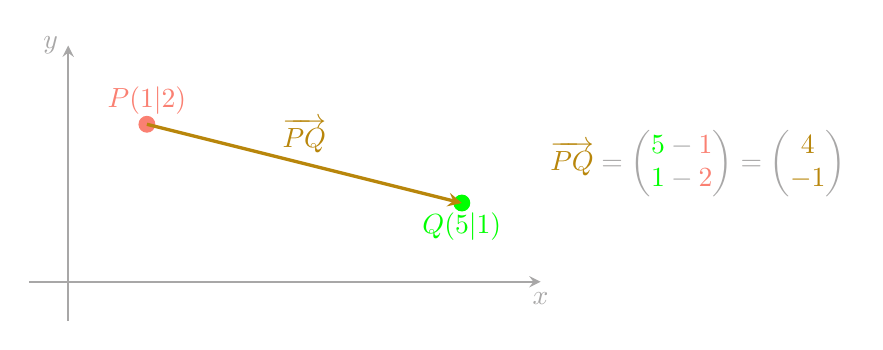
\begin{tikzpicture}[pfeil]

    \draw[thick, -stealth] (-0.5, 0) -- (6, 0) node[below] {$x$};
				\draw[thick, -stealth] (0, -0.5) -- (0, 3) node[left] {$y$};
				
				\draw[salmon, fill] (1, 2) circle (0.1) node[above] {$P(1|2)$};
				\draw[green, fill] (5, 1) circle (0.1) node[below] {$Q(5|1)$};
				
				\draw[darkgoldenrod, very thick, -stealth] (1, 2) -- node[above] {$\overrightarrow{PQ}$} (5, 1);
				
				\node at (8, 1.5) {$\color{darkgoldenrod}\overrightarrow{PQ}\color{pfeil}=\begin{pmatrix} \color{green}5\color{pfeil}-\color{salmon}1 \\ \color{green}1\color{pfeil}-\color{salmon}2 \end{pmatrix}=\begin{pmatrix} \color{darkgoldenrod}4  \\ \color{darkgoldenrod}-1 \end{pmatrix}$};

\end{tikzpicture}

\end{document}
